
\chapter{Overview about vector fields and segmentation techniques}
\section{The vector field}
What is a vector field? A Vector field is an assignment of a vector to each point in a subset of space. This assignment is the value that will gives an orientation to the row that will describe our image.
\begin{figure}
	\centering
	\begin{subfigure}[b]{0.5\textwidth}
        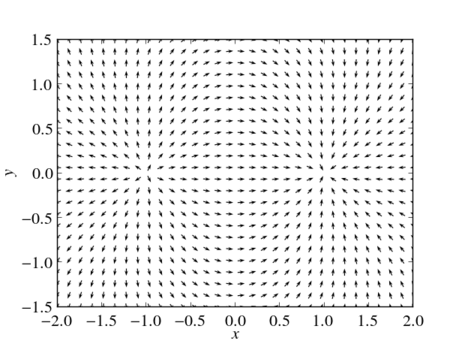
\includegraphics[width=\textwidth]{img/fieldex.png}
        \caption{ }
        \label{fig:field}
    \end{subfigure}
    \begin{subfigure}[b]{0.5\textwidth}
		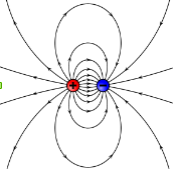
\includegraphics[width=\textwidth]{img/dipole.png}
		\caption{ }
		\label{fig:dipole}
	\end{subfigure}
	\caption{(a) Dipole electric field, (b) Electric dipole}
	\label{fig:fielddipole}
\end{figure}
The figure \ref{fig:fielddipole} represent a vector field flow of an electric dipole \ref{fig:dipole} in the $x-y-plane$ with $r+=(-1,0,0) $ and $ r-=(1,0,0)$. All vectors are normalized to the unity. Thus, the plot visualizes the direction of the electric dipole field, but not the field strength. In the negative zone part of the dipole it is possible to see that rows of the vector field tries to enter the plane and at the opposite side it’s possible to see the exact opposite, that shows the rows exit from the plane. This translates into a flow of rows that is possible to apply to describe the leukocyte's edges.

\bigskip


Active contours, also called snakes, are curves that move inside the image following the energy of the field. There are two kinds of forces, one internal and another external. Combining these two it's possible to create a curve that follows constraints gives by the forces. The  internal  and  external  forces  are  defined  so  that  the  snake  will conform to an object boundary or other desired features within an image. Snakes are widely used  in  many  applications,  including  edge  detection,  shape  modelling and segmentation. There  are  two  general  types  of  active  contour  models  in  the literature  today:  parametric active contours and geometric active contours. Typically,  the  curves  are  drawn  toward  the edges  by  potential  forces,  which  are  defined  to  be  the  negative  gradient  of  a  potential function.  Additional  forces,  such  as  pressure  forces,  together  with  the  potential  forces comprise the external forces. There are also internal forces designed to hold the curve together and to keep it from bending too  much.  There  are  two  levels  difficulties  with  active  contour  algorithms.  First,  the  initial contour must be close to the true boundary or else it will likely converge to the wrong result. The second problem is that active contours have difficulties progressing into concave  boundary  regions.  Although  many  methods  such  as  multi resolution  methods, pressure forces, distance potential forces, control points, and using solenoidal external fields have been proposed they either solve one problem or solve both but creating new difficulties. For  example,  multi resolution  methods  have  addressed  the  issue  of  initialization,  but specifying  how  the  snake  should  move  across  different  resolutions  remains  problematic. Another example is the pressure forces, which can push an active contour into boundary concavities, but cannot be too strong or “weak” edges will be overwhelmed. But how works a snake if the objects to segment are overlapped? Snakes are able to find all the external edges of the object but in this case the edge can be consider an internal part of the object. With the active contours is impossible segment the overlapped cells because the snake cannot enter inside the cell region. For these reasons we have used our virtual field following another lecture key. We use it only to exalt the edges of the cells in order to extract them.

\section{An overview about Image Segmentation methods}
When we talking about segmentation we introduce a technique for partitioning the image into subregions. Below are described the most five famous techniques to develop an image segmentation:
\begin{enumerate}
	\item threshold-based;
	\item histogram-based;
	\item region-based;
	\item edge detection;
	\item watershed transformation.
\end{enumerate}

\subsection{threshold-based techniques}
Thresholding is the simplest segmentation method. The pixels are partitioned depending on their intensity value generally used with gray scale images $f(x,y)$. When the threshold is apply on gray scale images the final target is separate the foreground by the background. The first one contains only the element of interest and the second one contains all the rest of the image. The global threshold value T is the 'breaking point' of the image. After an analysis of the image, the value T is used to understand if, taking in account each pixel of the image, each one it belongs to the foreground $f(x, y) > T$ or to the background $f(x, y) < T$ .It is used to understand if, taking in analysis each pixel of the image, it belows to the foreground $f(x, y) > T$ or to the background$f(x, y) < T$.\cite{Threshold}

\subsection{Histogram-based techniques}
An important class of point operations is based upon the manipulation of an image histogram or a region histogram. It uses the histogram to select the gray levels for grouping pixels into regions. The image is composed by the foreground and the background. Generally the background occupies most of the image and for this reason it's gray level will be a large peak in the histogram. The object of the image as opposed to the background is a smaller peak in the histogram. Then we can choose a threshold point in the valley between the two peaks and threshold the image.

\subsection{Region-based techniques}
Differently from the other two techniques described before, the region-based segmentation is a technique for determining the region directly. Initially set of point of interest are created. Starting from these points other regions grow up if neighbouring pixels have similar properties as that of point of interest. In region splitting and merging, an image is subdivided into different regions and then either merged and split. As first step the image is split into four disjoint quadrants, then merges any adjacent regions, which satisfy the imposed constraints. Like a loop we repeat splitting of regions and merging till no further merging or splitting is
possible. Image regions are implemented with the help of quad trees.
The basic formulation is:$\\
(a){\text{ }}\bigcup \nolimits _{{i=1}}^{{n}}{R_{{i}}=R.}\\
(b){\text{ }}R_{{i}}{\text{ is a connected region}},{\text{ i}}={\text{1}},{\text{ 2}},{\text{ }}...,{\text{n}}\\
(c){\text{ }}R_{{i}}\bigcap R_{{j}}=\varnothing\\
(d){\text{ }}P(R_{{i}})=TRUE{\text{ for }}i=1,2,...,n.\\
(e){\text{ }}P(R_{{i}}\bigcup R_{{j}})=FALSE{\text{ for any adjacent region }}R_{{i}}{\text{ and }}R_{{j}}\\
$

$P(R_{{i}})$ is a logical predicate defined over the points in set $R_{i}$ and $\varnothing$  is the null set.
(a) Means that the segmentation must be complete; that is, every pixel must be in a region.
(b) Requires that points in a region must be connected in some predefined sense.
(c) Indicates that the regions must be disjoint.
(d) Deals with the properties that must be satisfied by the pixels in a segmented region. For example, $P(R_{{i}})={\text{TRUE}}$ if all pixels in $R_{i}$ have the same gray-scale.
(e) Indicates that region $R_{i}$ and $R_{{j}}$ are different in the sense of predicate $P$.\cite{website:region_g}

\subsection{Edge detection technique}
Edge detection includes a variety of mathematical methods that aim at identifying points in a digital image at which the image brightness changes sharply or, more formally, has discontinuities. The points at which image brightness changes sharply are typically organized into a set of curved line segments termed edges. The same problem of finding discontinuities in one-dimensional signals is known as step detection and the problem of finding signal discontinuities over time is known as change detection. Edge detection is a fundamental tool in image processing, machine vision and computer vision, particularly in the areas of feature detection and feature extraction.\cite{edge} Is possible to divide Edges in two different set: intensity edges and texture edges. The first one includes steps and roofs. The Texture edges set include all the regions that are invariant to the luminance conditions. Then to obtain a continuous edge is necessary a function of edge linking. Below there are the most famous edge detection algorithms: Sobel, Prewitt, log, zero-cross, Roberts, Canny.

\subsection{Watershed technique}
This function considers the magnitude of the image like a topographic surface. We can consider it like an high ground of a gray-scale image, where the gray level of a pixel shows its height in the high ground. In proximity of the watershed lines the pixels have an high magnitude intensity. The water is put inside the regions enclosed by the watershed lines. As is possible to understand from these lines we are talking about a local minimum. We said it because for each region we find the local minimum and we fill it with the water. The result is composed only by the max-points of the image.

\bigskip

Next chapter illustrates, in detail, how we use the Mean Shift segmentation technique and the use of it's result with the VFC.